% INTRODUÇÃO-------------------------------------------------------------------

\chapter{INTRODUÇÃO}
\label{chap:introducao}

Dutos de ventilação usados nos sistemas de ar-condicionado estão sujeitos a diversos tipos de danos, dentre os quais pode-se listar os entupimentos progressivos devido ao acúmulo de poeira e de pequenos animais mortos. \citeonline{carmo1999qualidade} Por normalmente ser locais de difícil acesso, apresentam dificuldades em sua manutenção, favorecendo a proliferação de bactérias e transmissão de vírus \citeonline{bortoletto2002contaminaccao}.\par
Subestações de energia elétrica, em grande parte das vezes, ficam expostas a intempéries, que causam oxidações em suportes, equipamentos e cabos. Sua inspeção oferece riscos a vida por expor o corpo humano a uma quantidade enorme de energia. Apesar de existir uma norma rigorosa para a realização de inspeções preventivas, acidentes com vítima ainda acontecem \citeonline{santos2012inspeccao}.\par
A inspeção de reservatórios de produtos químicos requer uma minuciosa análise estrutural, uma busca por áreas oxidadas e falhas em pontos de solda, tarefa que demanda muitas horas de trabalho humano. A exposição a gases e vapores tóxicos, por menor que seja a quantidade, causam riscos a saúde do inspetor \citeonline{molina2008metodo}.\par
Os casos citados, são apenas algumas das atividades extremamente necessárias no ambiente industrial, que expõem a saúde das pessoas a riscos que poderiam ser evitados, através do uso de dispositivos especializados. \par 
Robôs equipados com ferramentas adequadas para cada tarefa, dotados de um sistema de navegação autônomo ou por controle remoto, podem ser usados para evitar ou minimizar os riscos a saúde dos inspetores. Como exemplo, o robô \textit{SENSABOT}, usado pela Shell, para monitorar e inspecionar plantas de óleo e gás, mostrado na \autoref{fig:sensabot}, e o robô \textit{ABB}, usado em inspeções de transformadores, sem a necessidade de drenar o óleo, visto na \autoref{fig:abb}. Contudo o uso de robôs não se restringe apenas ao ambiente industrial. No ano de 2011, robôs submarinos foram protagonistas na localização e resgate das peças do avião da Air France 447, que caiu no Oceano Atlântico em 2009. Foram usados robôs de inspeção, para verificar as condições estruturais da usina nuclear de Fukushima Daiichi no Japão, que foi afetada por um tsunami. 

\begin{figure}[H]
	\centering
	\begin{subfigure}{.5\textwidth}
		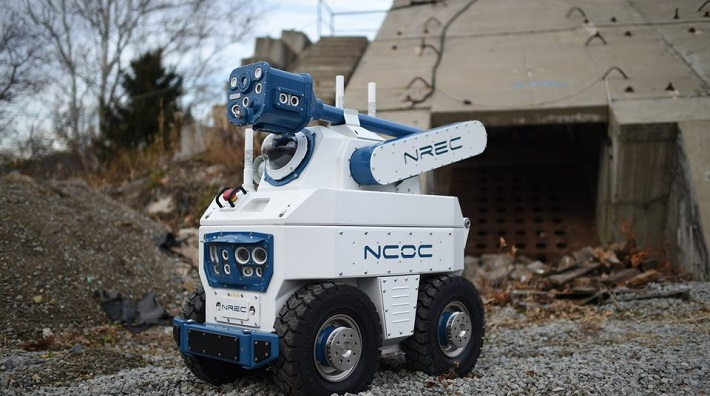
\includegraphics[width=0.95\textwidth]{figuras/sensabot.jpg}
		\caption{SENSABOT}
		\fonte{\citeonline{tractica2019sensabot}.}
		\label{fig:sensabot}
	\end{subfigure}%
	\begin{subfigure}{.5\textwidth}
		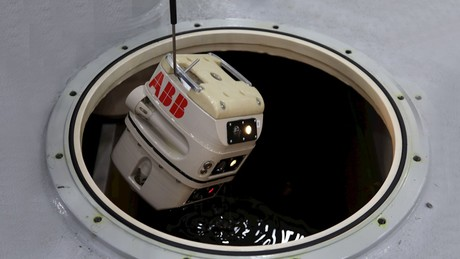
\includegraphics[width=0.95\textwidth]{figuras/abb.jpg}
		\caption{ABB}
		\fonte{\citeonline{processonline2019abb}.}
		\label{fig:abb}
	\end{subfigure}
	\caption{Robôs de inspeção}
\end{figure}

Independente de um robô ser controlado diretamente por uma pessoa, ou operar em modo completamente autônomo, em algum momento, a observação, supervisão e o julgamento humano ainda é um elemento crítico da atividade robótica.\par

A maior ligação perceptual entre um ambiente remoto e o operador de um robô, acontece através do vídeo enviado por uma (ou mais) câmera montada no robô. Existe uma relação forte entre problemas de localização da câmera e sua montagem, bem como angulo de visão e outros fatores, que podem degradar essa ligação e deixar o operador vulnerável a uma serie de erros como: desorientação, falha ao reconhecer danos ou simplesmente não notar um ponto importante durante uma inspeção.\par

Estudos sugerem que disponibilizar uma câmera controlada independentemente da orientação de um robô, pode facilitar tarefas de localização num ambiente. \citeonline{hughes2004robotic}

A complexidade de operação de um robô é proporcional ao seu DOF (\textit{Degrees of Freedom}), isto é, quanto maior a variedade de movimentos o robô pode executar (considerando seu deslocamento, movimento de braços mecânicos e câmera), mais difícil é o controle manual para o operador.
Pensando nisso, o desenvolvimento de controles mais intuitivos para a câmera embarcada, diminui a complexidade geral do controle de movimentos globais do robô. \par

Com o objetivo de aprofundar os conhecimentos adquiridos ao longo do curso, este trabalho visa criar um controle de câmera do tipo \textit{Pan} e \textit{Tilt}, baseando-se nos dados de movimento, coletados e enviados, através de rede sem fio, por um \textit{smartphone} acoplado a cabeça do operador, por um óculos VR (\textit{Virtual Reality}). Dessa forma, os movimentos de rotação da cabeça do operador (\textit{yaw} e \textit{pitch}) são traduzidos em movimentos da câmera (\textit{Pan} e \textit{Tilt}), montada no robô. \par 

No projeto, pretende-se utilizar um \textit{Raspberry Pi}, como unidade computacional e de controle dos servo motores da câmera, e um celular \textit{smartphone} \textit{Android}, responsável por coletar e enviar informações referentes a posição espacial do aparelho. \par

Com o desenvolvimento do projeto procura-se um melhor entendimento em aspetos relacionados a rede de computadores, sistemas operacionais, interfaces de hardware, modulação por largura de pulso, eletrônica geral e desenvolvimento de sistemas para plataformas móveis.\par

Competências ligadas a construção de software, utilizando múltiplas linguagens de programação, devem ser evoluídas, já que o módulo de controle, embarcado no \textit{Raspberry Pi}, deve ser construído em linguagem C e o módulo de coleta de dados desenvolvido em Java, usando a API (\textit{Application Programming Interface}) fornecida pelo sistema operacional \textit{Android}.\par

